\chapter{PROBLEM DEFINITION}
\label{chapter:problem}
\hyphenation{BeamCal}
\section{The BeamCal Instrumentation }

The work described in this thesis is a contribution to the design and implementation of the front-end circuit for one of the detector systems of the International Linear Collider (ILC). The project is endorsed by the ILC Forward Calorimetry Collaboration (FCAL), a worldwide detector research and development collaboration, and party sponsored by CONICYT through the FONDECYT Program.

Planned to be operating in the mid 2020’s, the ILC will be the largest linear particle collider ever built. Consisting of two linear accelerators that will stretch approximately 32 kilometers in length, the ILC will smash electrons and positrons together at nearly the speed of light. The intended beam collision energy is 500 billion-electron-volts (GeV) for the first stage, with the possibility for a later upgrade to 1 TeV. 
 
Located at the ILC detector forward region, the BeamCal is a highly segmented \mbox{($>$ 90000 channels)} calorimeter that will serve four main purposes: improve the hermeticity of the ILC detector for low polar angles, reduce the backscattering from pairs into the inner ILC detector part, protect the final magnet of the beam delivery system, and assist the beam diagnostics. The BeamCal specifications for radiation tolerance, noise, signal charge, pulse rate and occupancy pose unique challenges for the instrumentation system. Although initially planned  for the ILC, the BeamCal calorimeter could also be used in the Compact Linear Collider (CLIC), the alternative particle accelerator in race to follow the LHC.

The FONDECYT project \#11110165: Application of Advanced CMOS Techniques in Pulse Processors for Particle Physics Experiments deals with the design and implementation of a mixed-signal application-specific integrated circuit (ASIC) to address the BeamCal instrumentation needs. The IC, called the Bean, will be designed for a standard 180-nm CMOS process and will be based on a 3-channel prototype developed in a previous work \citep{abusleme101}. Each independent channel will include: a charge-sensing amplifier with a pre-charging pulser; a fully differential switched-capacitor (SC) filter with a low-frequency noise suppression feature; a 10-bit, fully-differential, successive approximation register (SAR) charge redistribution analog-to-digital converter (ADC); and a digital storage array. Additionally, the IC will feature a fast feedback adder for beam diagnostics purposes. Fig.~\ref{fig:bean_diag} shows a block diagram of a prototype version of the Bean, which does not include the digital storage array nor the nominal number of channels. The IC will be capable of processing the BeamCal detector output at the ILC nominal frequency of $3.2468\,\text{MHz}$, with 100\% occupancy\footnote{Occupancy is the fraction of channels that register a relevant stimulus on each collision.}. Also, each channel must be able to deal with  two different modes of operation: the standard data taking (SDT) mode, and the detector calibration (DCal) mode. According to the actual BeamCal specifications, the maximum input signals were to be about 37 pC in the SDT mode, and 50 times smaller in the DCal mode. Table~\ref{tab:bean_specs} summarizes the BeamCal instrumentation ASIC specifications. 

Beyond the purpose of addressing the BeamCal instrumentation needs, the general goal of this project is to prove that advanced CMOS circuit design techniques, such as SC circuits and ADCs based on MOM capacitors, can be used effectively to address the instrumentation requirements in particle physics experiments. 
The specific goals of this project to be covered by this thesis are:
\begin{enumerate}
\item  to achieve a thorough understanding of the noise of SC filters in particle physics experiments, and
\item  to prove the successful synthesis of arbitrary WFs by means of SC circuits.
\end{enumerate}

The first goal is sorted out with the development of a mathematical framework for noise analysis in discrete-time filters presented on Chapter \ref{chapter:theoretical}, which is not only suited for SC filters, but for any discrete-time block introduced on the signal path of the circuit in analysis.

The second goal is carried out by means of the implementation of the front-end filter for the Bean, which development is shown in Chapter \ref{chapter:filter}.

\begin{figure}[!t]
	\centering
	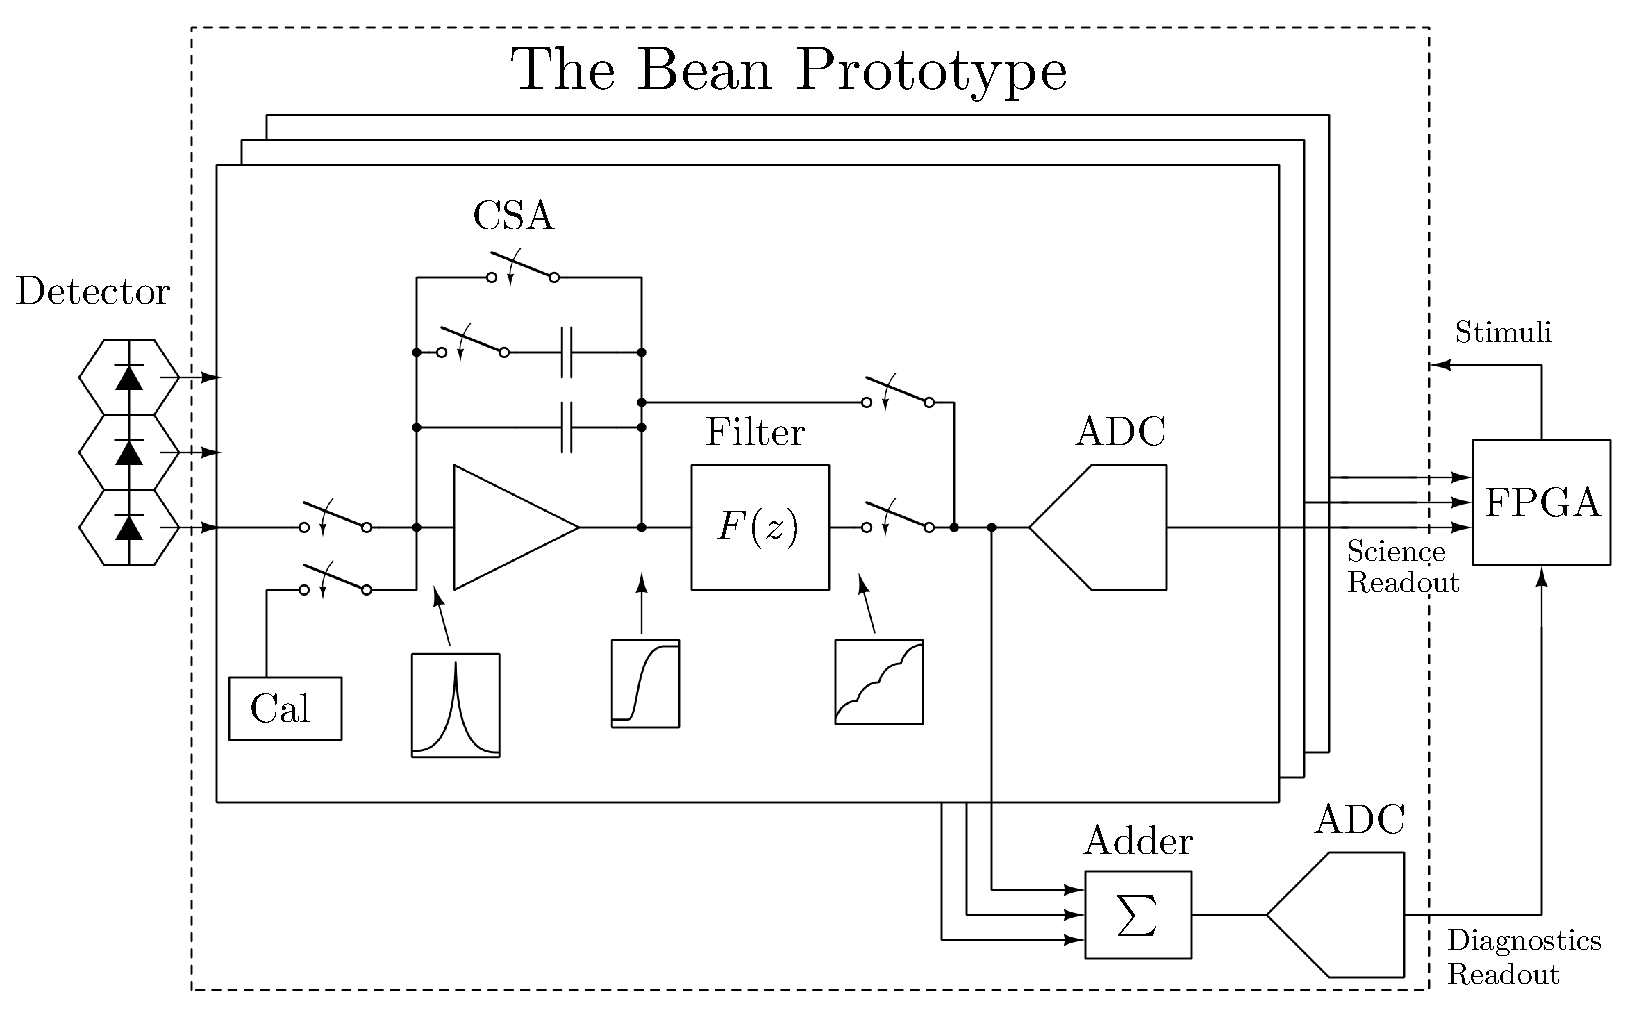
\includegraphics[width=5.3in]{./Figures/thebean_diag.eps}
	\caption{The Bean prototype block diagram.}\label{fig:bean_diag}
\end{figure}

\begin{table}[!t]
	\begin{center}
		\begin{tabular}{|l|l|}\hline
			Input rate & $3.25\,\text{MHz}$ during $0.87\,\text{ms}$, repeated every $200\,\text{ms}$ \\ \hline
			Channels per ASIC & $32$ \\ \hline
			Occupancy & $100\%$ \\ \hline
			Resolution & $10$ bits for individual channels, $8$ bits for fast feedback \\ \hline
			Modes of operation & Standard data taking (SDT), Detector Calibration (DCal) \\ \hline
			Input signals & Up to $40$ pC in SDT, $0.74$ pC in DCal \\ \hline
			Input capacitance & $65$ pF \\ \hline
			Additional feature & Low-latency ($1\,\micro\text{s}$) output \\ \hline
			Additional feature & Internal pulser for electronics calibration \\ \hline
			Radiation tolerance & 1 Mrad ($\text{SiO}_2$) total ionizing dose \\ \hline
			Power consumption & $2.19$ mW per channel \\ \hline
			Total ASIC count & $2836$ \\\hline
		\end{tabular}
		\vspace*{5pt}
		\caption{BeamCal instrumentation ASIC specifications summary.}\label{tab:bean_specs}
	\end{center}
\end{table}